\chapter{Environment and algorithms}
\label{ch:algo}

This chapter gives a description of the environment and the algorithms that
were used in the experiment described in chapter \ref{ch:method}. The environment Invasive Species, is a simulation of a river network with invading species where to goal is to eradicate unwanted species and is further described in section \ref{sec:experiment_env}. 

Two algorithms are covered in this chapter, both of which deal with the
problems that arise with large state spaces; however, they differ in the
methods they apply. In the following chapter the general ideas behind the
algorithms, as well as specific details, are presented. 

The model-based interval estimation algorithm, described in
section~\ref{sec:mbie}, utilizes clever estimations of confidence intervals for
the Q-value functions to improve performance in sparse MDPs.
Section~\ref{sec:fac_e3} is on an algorithm that uses dynamic bayesian networks
and factored representations to improve the \etre\ algorithm to efficiently
deal with factored MDPs. 

\section{Environment specification, Invasive Species}
\label{sec:experiment_env}

When the agents were tested, the Invasive Species environment from the 2014 edition of
the Reinforcement Learning Competition was used. The environment is a
simulation of an invasive species problem, in this case a river network with
invading species where the goal of the agent is to eradicate unwanted species
while replanting native species. 

The environment's model of the river network has parameters, such as the size
of the river network and the rate at which plants spread, which can be
configured in order to create different variations of the environment.  The
size of the river network is defined by two parameters: the number of reaches
and the number of habitats per reach. A habitat is the smallest unit of land
that is considered in the problem. A habitat can either be invaded by the
tamarix, which is an unwanted species, empty or occupied by native species. A
reach is a collection of neighboring habitats. The structure of the river
network is defined in terms of which reach is connected to which
\parencite{invasiveSpecis2014:Online}. In figure \ref{fig:river} a model of a
river network is shown.

\begin{figure}[ht]
\centering
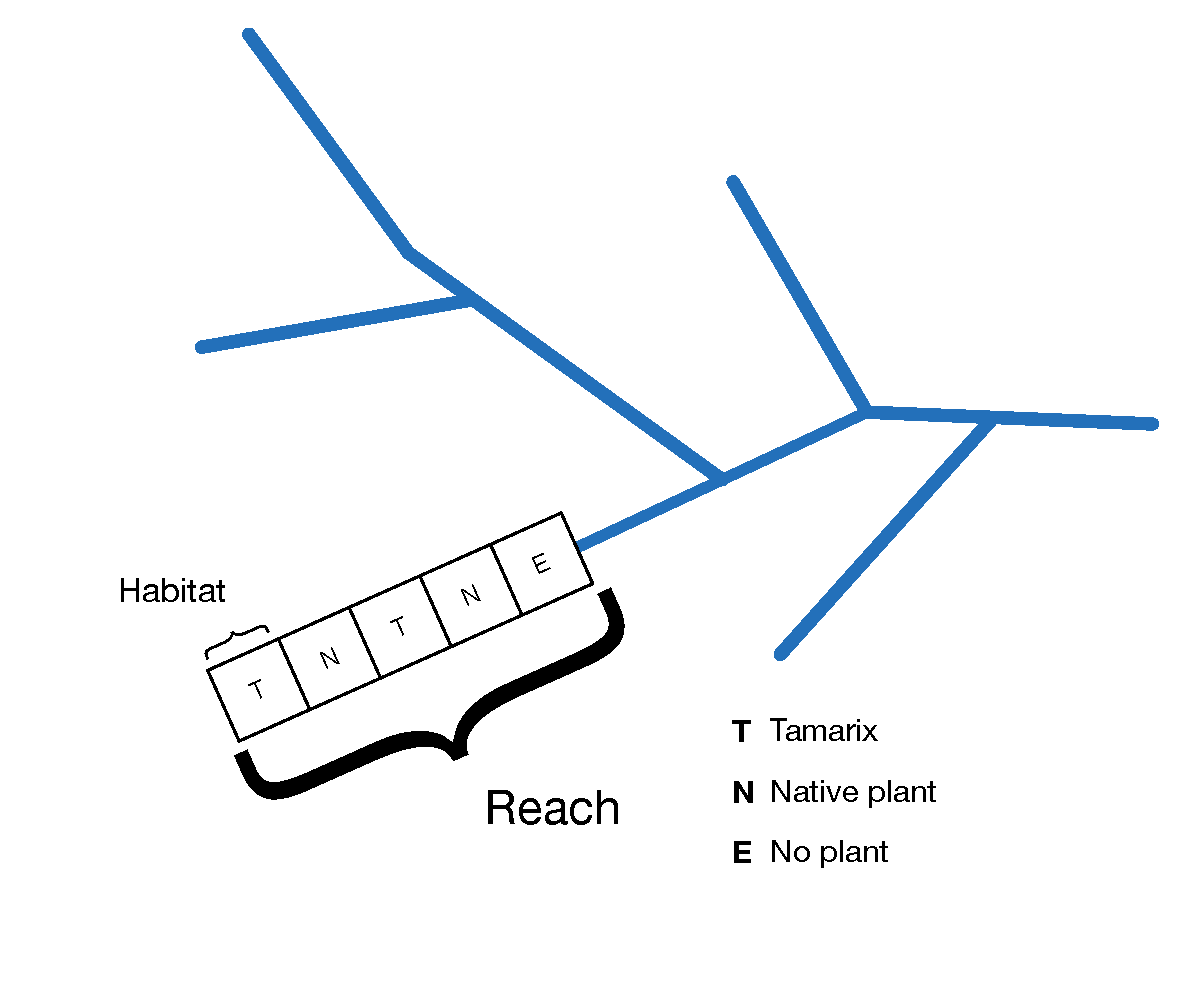
\includegraphics[width=0.9\textwidth]{images/river_network.pdf}
\caption{A river network, as modeled by the Invasive Species reinforcement learning environment.}
\label{fig:river}
\end{figure}

There are four possible actions (eradicate tamarix trees, plant native trees,
eradicate tamarix trees and plant native trees and a wait-and-see action),
and the agent chooses one of these actions for each reach and time step. If the 
agent chooses to eradicate tamarix trees or plant native trees in a reach, 
all habitats of that reach are targeted by this action. What
actions are available to the agent depends on the state of each reach. It is
always possible to choose the wait-and-see action, but there has to be one
or more tamarix-invaded habitats in a reach for the eradicate or eradicate and
plant actions to be available and there has to be at least one empty habitat in
a reach for the plant-native-trees action to be available
\parencite{invasiveSpecis2014:Online}.  

\section{Model-based interval estimation}
\label{sec:mbie}

Model-based interval estimation is a modification of value iteration whose main feature is its  addition of confidence
intervals to the state-action values. These confidence intervals allow the agent to choose between
actions, based on how confident it is about its evaluation of them. In effect,
the less certain the agent is about its evaluation of the states and actions,
the more exploratory the actions will be. When the agent is more confident
however, it will exploit what it has learnt so far about the MDP
\parencite{dietterich2013pac}.


\subsection{Optimistic estimations of transition probabilities}
\label{sec:computep}

The first step of the MBIE algorithm is to find optimistic estimations of transition probabilities. Equation \eqref{equation:balls_of_steels} describes, as a set, the confidence interval (CI) used by MBIE for the probability distribution over destination states when taking action $a$ in state $s$. So, the first task of the algorithm is to find the element within this set that is maximally optimistic, meaning that it gives the best value to $(s,a)$ in the following value-iteration step of the MBIE algorithm. A description of how this is done in practice is described in section \ref{sec:ptilde}. 

In equation \eqref{equation:balls_of_steels}, $\hat{P}$ is the observed probability distribution (treated as a vector) for destination states from $(s,a)$, $N(s,a)$ is the number of times that the state-action pair $(s,a)$ has been observed, $\delta$ is a confidence parameter,  $\omega$ is a value given by \eqref{equation:omega} and $\|x\|_1$ denotes the l1-norm of the vector $x$. The l1-norm is the sum of the absolute value of all elements of a vector. 

\begin{equation}
\label{equation:balls_of_steels}
CI\left(\hat{P} \left| N(s, a), \delta\right.\right)  = \left\{\tilde{P} \left| \|\tilde{P} - \hat{P}\|_1 \le \omega(N(s,a), \delta), \|\hat{P}\|_1 = 1, \hat{P}_i \geq 0  \right.\right\}
\end{equation}

\begin{equation}
\label{equation:omega}
   \omega(N(s,a),\delta) = {\sqrt{\frac{2|ln(2^{|S|}-2) - ln  \delta |}{N(s,a)}}}
\end{equation}

In equation \eqref{equation:omega}, $\omega(N(s,a),\delta)$ gives a bound for how much the vector of transition probabilities can be changed from the observed values, while remaining within the confidence interval. In this equation, $|S|$ is the number of states in the MDP and the other variables have the same meaning as in \eqref{equation:balls_of_steels}. For the derivation of this formula, see  \textcite{Strehl20081309}.

\subsection{Compute$\tilde{P}$}
\label{sec:ptilde}
The method for finding the sought element within the set denoted by \eqref{equation:balls_of_steels} 
is refered to as Compute$\tilde{P}$ in this report. 
The fundamental idea of the Compute$\tilde{P}$ method is that it starts with
the observed transition probabilities $\hat{P}$ and then it moves probability
mass from ``bad'' outcomes to ``good'' outcomes and finally returns the resulting probability distribution, $\tilde{P}$. 


\paragraph{Initialization} The state transition probability distribution is initialized according to
\eqref{equation:roof}, which corresponds to the observed probabilities.

\begin{equation}
\label{equation:roof}
\tilde{P}(s'|s, a) := \hat{P}(s'|s, a) = \frac{N(s,a,s')}{N(s,a)}
\end{equation}

In \eqref{equation:roof}, $N(s, a)$ is the number of times action $a$ has been taken in
state $s$ and $N(s, a, s')$ is the number of times action $a$ has been taken in
state $s$ and the agent ended up in state $s'$.

\paragraph{Moving probability mass} The procedure of moving probability mass is done by first finding the outcome
state with the best $V$-value and observed probability less than 1, calling it
$\overline{s}$. Analogously the outcome with the worst $V$-value with an
observed probability of greater than 0 is found, and this state is called
$\underline{s}$. If a $V$-value has not been computed yet for a certain state, it is 
assumed to have the maximum possible value. 

The probability values $\tilde{P}(\underline{s}|s,a)$ and
$\tilde{P}(\overline{s}|s,a)$ are then increased or decreased according to
equations \eqref{equation:ptilde_floor} and \eqref{equation:ptilde_roof}.

\begin{equation}
\label{equation:ptilde_floor}
\tilde{P}(\underline{s}|s,a) := \tilde{P}(\underline{s}|s,a)-\xi
\end{equation}

\begin{equation}
\label{equation:ptilde_roof}
\tilde{P}(\overline{s}|s,a) := \tilde{P}(\overline{s}|s,a)+\xi
\end{equation}

Since the sum of the probabilities needs to equal one and 
no single transition probability may fall below zero or exceed one, the probability distribution can only be modified by at most $\xi$, as given by
equation \eqref{equation:xi}, where $\Delta\omega = \omega / 2$. The variable $\Delta\omega$ denotes the total mass that can be moved, without $\tilde{P}$ having a lower chance than $1 - \delta$ of being within the confidence interval for the probability distribution. If $\xi$ is less than $\Delta \omega$, new states
$\overline{s}$ and $\underline{s}$ are found, and probabilities are moved until
mass equal to $\Delta \omega$ has been moved in total or the probability mass has all been moved to an optimal state. 

\begin{equation}
\label{equation:xi}
\xi = \min\{
  1 - \tilde{P}(\overline{s} | s, a)
  , \tilde{P}(\underline{s} | s, a)
  , \Delta \omega 
\}
\end{equation}


\label{goto}



\subsection{Value iteration with confidence intervals}
\label{sec:modification_conf_interval}
When Compute$\tilde{P}$ has been run, the resulting $\tilde{P}$ is used in a standard value
iteration, as in \eqref{equation:q_upper}. Thus, Compute$\tilde{P}$ finds the probability distribution that maximizes the sum in this equation. 

Finally, optimistic state values are computed according to \eqref{equation:vMBIE}. These values are simply the value of the best action for each state. These values are used the next time that Compute$\tilde{P}$ is run and ``good'' and ``bad'' states need to be found. 

\begin{comment}
The confidence  bounds on the Q-values in the MBIE-algorithm are calculated by
making a maximally optimistic estimation of these values, given some confidence
parameter. The less times a state-action pair has been visited, the more
optimistic this estimation will be. This has the effect of promoting
exploration of actions that have been taken few times. 

When a state is first encountered by the agent, the Q-values associated with
the state are initialized with the maximum achievable reward. When the actions
are later performed, the state-action pairs have their Q-values gradually
decreased depending on the expected value. Given time, the confidence bounds will
become smaller and smaller, and the policy will converge to optimal actions
with confidence specified by a confidence parameter. The bound for the
confidence interval on a Q-value can be calculated by iterating the following
equation (cf. section~\ref{sec:valueiteration} about the basic value iteration
algorithm) for all state-action pairs until it converges:
\end{comment}

\begin{align}
\label{equation:q_upper}
Q_{upper} (s, a) = & R(s, a) + \nonumber \\
& \operatorname*{max}_{\tilde{P}(s, a)\in CI(P(s, a), \delta)} \gamma \sum_{s'} \tilde{P}(s'|s, a)\operatorname*{max}_{a'} Q_{upper}(s', a')
\end{align}


\begin{equation}
\label{equation:vMBIE}
V_{upper}(s) = max_aQ_{upper}(s,a)
\end{equation}

\subsection{Optimizations based on Good-Turing estimations}

\label{sec:mbie_gt}

One problem with the method described above is that probability mass can be
moved to any outcome state, without any consideration taken as to whether this
outcome has ever been observed. \textcite{dietterich2013pac} make
use of an optimization that deals with this by limiting the probability mass
that can be moved to outcomes that have never been observed. The limit that is used is the approximation
of the probability mass in unobserved outcomes as estimated by Good and Turing
as $\hat{M}_0(s,a) = |N_1(s,a)| / N(s,a)$ \parencite{gtpaper}. In this
equation, $N_1(s,a)$ is a set of the states that have been observed exactly
once as an outcome when taking action $a$ in state $s$ and $N(s,a)$ is the
number of times that action $a$ has been taken in state $s$ in total. 
\subsection{Implementation choices and extensions for MBIE}
\label{sec:MBIE_our_contribution}

\paragraph{How often to perform planning}
\label{sec:mbie_perform_planning}

It is possible to perform planning and compute a new policy once for each
action taken by the agent. However, this would be unnecessarily slow to
compute. The planning comprises iterating Q-value updates to convergence and
then using these converged values to update V-tables, a considerable number of
computations. So instead of planning after every action taken, the algorithm
only performs planning and updates the policy at some given interval. 

A way to do this that we have used is to only perform an update when the number 
of visits to a specific state-action pair has doubled. This is
done for small variants of the Invasive Species environment. For large variants
we perform planning when the total number of actions taken has been multiplied
by 1.5. A large variant is defined as when the number of state variables
exceeds 9. This number was determined by running some preliminary tests and
choosing a number giving a reasonable run time.

\paragraph{Optimizing bounds}

Another optimization that can be performed is that the value $\Delta \omega$ in
equation~\eqref{equation:xi} can be tweaked to fit the environment that the
agent is used with. Equation \eqref{equation:xi} gives bounds for which it can
be proved that the method always converges to an optimal policy. In practice,
however, this value can be reduced by quite a bit in order to speed up the rate
at which the agent considers state-action pairs known. 

A simple linearly declining function can be used instead of
equation~\eqref{equation:xi}. In the so called realistic implementation of MBIE we have
used $\omega = 1 - \alpha N(s,a).$ The value of the $\alpha$ parameter was decided through experimentation (see section \ref{sec:test_spec}).



\section{\etre\ in factored Markov decision processes}
\label{sec:fac_e3}

The second algorithm studied in this thesis is a version of the \etre\ algorithm that focuses on factored problem domains by modeling them as a dynamic Bayesian network. The original \etre\ algorithm is described in section \ref{sec:e3}, which gives a broad overview along with the key strategies used in the algorithm. The following section, \ref{sec:factored_e3}, considers some ways to extend the original algorithm and make use of factored representations and planning in factored domains to improve the running time of the algorithm.

\subsection{The \etre\ algorithm}
\label{sec:e3}

\etre\ (Explicit Explore or Exploit) is an algorithm that divides the state space into two parts --- known states and unknown states --- in order to decide whether it is better to explore unknown states or to exploit the agent's knowledge of the known states. A state is considered to be known if the \etre\ agent has visited it enough times. All other states are either unknown or have never even been visited. Unknown and unvisited states are treated in the same way. In the following sections a description is given of the three phases of operation of \etre\, which are called balanced wandering, exploration and exploitation \parencite{kearns2002near}.

\paragraph{Balanced wandering}

When the agent finds itself in a state that it has not visited a large enough number of times to be considered a known state, it enters a phase called balanced wandering. When in balanced wandering, the agent always takes the action performed from this state the least number of times. 


\paragraph{Exploration}
When the agent from the balanced wandering phase enters a state that is known, it performs a policy computation to find a policy that maximizes the agent's chance of ending up in an unknown state. 

This exploration policy calculation is performed on an MDP which contains all known states and their experienced transition probabilities. 
All unknown states are gathered in a super-state with transition probability 0 to all known states and 1 to itself. The rewards are set to 0 for known states whereas the reward for the super-state is set to the maximum possible reward. A policy based on this MDP definition will strive to perform actions that reach the super-state, i.e., an unknown state.

If the chance of ending up in the super-state is below a certain threshold, it can be proved that the agent knows enough about the MDP that it is probable that it will be able to calculate a policy that is close to optimal \parencite{kearns2002near}.

\paragraph{Exploitation}
Inversely, if the agent's chance of being able to explore is low enough, it performs a policy computation in order to find a policy that maximizes rewards from the known part of the MDP. This exploitation policy computation is performed on an MDP comprising all known states, their observed transition probabilities and their observed rewards. A super-state representing all unknown states is also added to the MDP with reward 0 and transition probability 0 to all known states and 1 to itself. This MDP definition will result in a policy that favors staying in the known MDP and finding a policy with high return.

\paragraph{Leaving the exploitation and exploration phases}
When the agent is in either the exploration or exploitation phase, there are two events that can trigger it to exit these phases. First, if the agent enters an unknown state, it goes back to the balanced wandering phase. Second, if it has stayed in the exploration or exploitation phase for $T$ time steps, where $T$ is the horizon time for the MDP, it goes back to the behavior described in the ``exploration'' section above.


%\subsection{Our contribution}
\subsection{Factored additions to \etre}
\label{sec:factored_e3}

The \etre\ algorithm does not exploit that the underlying Markov Decision
Process may be structured in a way that allows certain optimizations. Therefore
\etre\ has a running time that scales polynomially with the number of states in
the MDP. However, by using a factored approach for the problem, improvements
can be made to the running time. By factoring the problem as a dynamic bayesian
network, the running time will scale with the number of random variables in the
underlying DBN instead for the number of states
\parencite{kearns1999efficient}. 

When using a factored representation some changes to the original algorithm are
required to make it compatible. One issue that has to be solved is how to
perform  planning with the new representation. In this thesis a modified version
of value iteration was used for planning and it is described later in this
section. In section \ref{sec:better_planing_algos} there are other methods
presented.


\paragraph{Dynamic bayesian network structure}

Assume that the states of an MDP each are divided into several variables. For
instance, the Invasive Species MDP described in section
\ref{sec:experiment_env} constitutes such a case, where the status of each
reach can be considered a variable on its own. The number of tamarix trees,
native trees and empty slots in a certain reach at time step $t+1$ depends not
on the whole state of the environment at time $t$, but only on the status of
adjacent reaches. Those variables on which another variable depend are called
its parents.  

An MDP that follows the description in the previous paragraph is described as
factored. With the assumption of a factored MDP, it is possible to describe its
transition probabilities as a dynamic bayesian network, where one would have a
small transition probability table for each of the reaches in the MDP, instead
of a large table for the transitions for the whole states.


